\documentclass[11pt]{article}
\usepackage[a4paper, portrait, margin=1in]{geometry}
\usepackage{listings}
\usepackage[dvipsnames]{xcolor}
\usepackage{color}
\usepackage{graphicx}
\usepackage[colorlinks=true,urlcolor=blue,linkcolor=gray]{hyperref}
% Fancy header package for version number

\usepackage{fancyhdr}
\pagestyle{fancy}
\fancyhf{}
\renewcommand{\headrulewidth}{0pt}
\renewcommand{\footrulewidth}{0pt}

\fancypagestyle{firstpagefooter}
{
\lfoot{Version: 29.09.2016}
\cfoot{}
\rfoot{\thepage}
}
\cfoot{\thepage}

\newcommand{\code}[1]{\lstinline[language=Java]{#1}}
\newcommand{\todo}[1]{\fcolorbox{black}{Apricot}{TODO: #1}}
\newcommand{\linkmain}[1]{\href{https://gitlab.inf.ethz.ch/pungast/asl-fall16-project/blob/master/src/main/java/asl/#1.java}{#1}}
\newcommand{\linktest}[1]{\href{https://gitlab.inf.ethz.ch/pungast/asl-fall16-project/blob/master/src/test/java/asl/#1.java}{#1}}

\newcommand{\footnotemain}[1]{\footnote{\url{https://gitlab.inf.ethz.ch/pungast/asl-fall16-project/blob/master/src/main/java/asl/#1.java}}}
\newcommand{\footnotetest}[1]{\footnote{\url{https://gitlab.inf.ethz.ch/pungast/asl-fall16-project/blob/master/src/test/java/asl/#1.java}}}

%\newcommand{\resultsurl}[1]{\url{https://gitlab.inf.ethz.ch/pungast/asl-fall16-project/blob/master/results/#1}}
\newcommand{\resultsurl}[1]{\href{https://gitlab.inf.ethz.ch/pungast/asl-fall16-project/blob/master/results/#1}{gitlab.inf.ethz.ch/.../results/#1}}

\begin{document}

\title{Advanced Systems Lab (Fall'16) -- First
Milestone}

\author{\textbf{Name: \emph{Taivo Pungas}}\\\textbf{Legi number: \emph{15-928-336}}}

\date{
\vspace{4cm}
\textbf{Grading} \\
\begin{tabular}{|c|c|}
\hline  \textbf{Section} & \textbf{Points} \\
\hline  1.1 &  \\ 
\hline  1.2 &  \\ 
\hline  1.3 &  \\ 
\hline  1.4 &  \\ 
\hline  2.1 &  \\ 
\hline  2.2 &  \\ 
\hline  3.1 &  \\ 
\hline  3.2 &  \\ 
\hline  3.3 &  \\ 
\hline \hline Total & \\
\hline 
\end{tabular} 
}

\maketitle
\thispagestyle{firstpagefooter}
\newpage


\section{System Description}\label{sec:system-description}

\subsection{Overall Architecture}\label{sec:desc:architecture}

The most important classes in this implementation all belong to the package \code{main.java.asl} and are as follows. Whenever a Java class is referenced, it will link to GitLab, e.g. \linkmain{MiddlewareMain}. 

\begin{itemize}
\item \linkmain{MiddlewareMain} is responsible for setting up all parts of the middleware, and creating the \code{ExecutorService} with a fixed thread pool of $(T+1) \cdot N + 1$ threads.
\item \linkmain{Request} is a wrapper class for all GET- and SET-requests.
\item \linkmain{LoadBalancer} is the front of the middleware. It reads all incoming requests from all clients using \code{java.nio}, hashes the requests using \linkmain{UniformHasher} and forwards them to the correct servers for writing or reading. More in Section~\ref{sec:desc:hashing}.
\item \linkmain{MiddlewareComponent} is a lightweight class that holds the read and write queues for a given server, and starts the threads that process requests from those queues.
\item \linkmain{WriteWorker} and \linkmain{ReadWorker} implement the write and read thread for a given \linkmain{MiddlewareComponent}. More in Sections~\ref{sec:desc:writes} and \ref{sec:desc:reads}.
\end{itemize}

\begin{figure}[h]
\centering
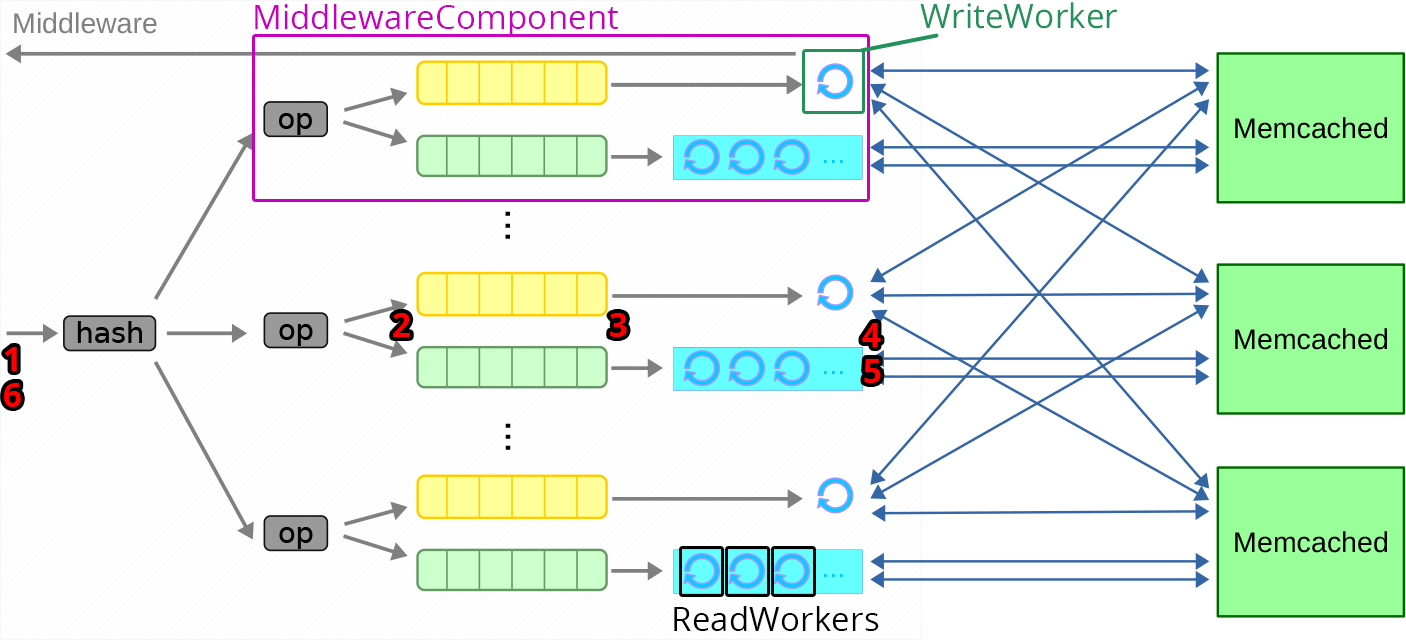
\includegraphics[width=0.8\textwidth]{figures/structure.png}
\label{fig:structure}
\caption{Middleware architecture.}
\end{figure}

The middleware is instrumented at six points that are also shown in Figure~\ref{fig:structure}:
\begin{enumerate}
\item $t_{created}$ -- when the request is received in \linkmain{LoadBalancer}.
\item $t_{enqueued}$ -- when the request is added to the queue.
\item $t_{dequeued}$ -- when the request is removed from the queue.
\item $t_{forwarded}$ -- when the request has been sent to all the servers (one server for GET requests and $R$ servers for SET requests).
\item $t_{received}$ -- when responses to the request have been received from all servers.
\item $t_{returned}$ -- when the response is returned to the client.
\end{enumerate}

\todo{"Shortly outline the main design decisions?"}

\subsection{Load Balancing and Hashing}\label{sec:desc:hashing}

The hashing is implemented by \linkmain{UniformHasher}. The hashing scheme for a given key works as follows:
\begin{enumerate}
\item s is hashed into a 32-bit signed integer $i$ using Java's native \code{String.hashCode()}.
\item The index of the primary machine is calculated as $i \bmod N$ (adding $N$ if the modulus is negative) where $N$ is the number of servers.
\end{enumerate}

The uniformity of hashing was also validated in tests (see \linktest{UniformHasherTest}). For 1 million random strings and 13 target machines, the distribution to different machines was the following:

\begin{verbatim}
Machine   0 got      77229 hits.
Machine   1 got      76702 hits.
Machine   2 got      76769 hits.
Machine   3 got      76860 hits.
Machine   4 got      76773 hits.
Machine   5 got      77169 hits.
Machine   6 got      76650 hits.
Machine   7 got      76831 hits.
Machine   8 got      77061 hits.
Machine   9 got      76955 hits.
Machine  10 got      76644 hits.
Machine  11 got      77432 hits.
Machine  12 got      76925 hits.
\end{verbatim}

As apparent, the distribution is indeed uniform.

Selection of replicated machines for a given replication factor $R$ was done by first selecting the primary machine using the scheme described above, and then selecting the next $R-1$ machines for replication. E.g. for a setup with 8 memcached servers and $R=5$, a key whose primary machine is 5 would be replicated to machines 6, 7, 0, and 1.

\subsection{Write Operations and Replication}\label{sec:desc:writes}

The write operations are handled by \linkmain{WriteWorker}s. Each \linkmain{WriteWorker} runs on one thread and has exactly one connection to each memcached server it needs to write to, so in total $R$ connections (where $R$ is the replication factor).

\linkmain{WriteWorker} runs an infinite while-loop in which it does two distinct things.

Firstly, if there are any requests available in the queue of SET-requests, it removes one request r from the queue. It then writes to each of the replication servers in a serial manner without waiting for a response, i.e. it writes the whole SET-request to the first server, then to the second server, and so on. For the non-replicated case, only one request is sent.

Secondly, \linkmain{WriteWorker} checks all memcached servers to see if any of them have responded. This is done in a non-blocking manner using \code{java.nio}: if a server is not yet ready to respond, other servers will be checked; if no server is ready to respond, the first step is run again. \linkmain{WriteWorker} keeps track of all responses to the same request and once all servers have returned a response, the worst out of the $R$ responses is forwarded to the client. For the non-replicated case, this process reduces to just forwarding the response from memcached to the client.


\todo{Estimate of latencies -- replicated and non-replicated}
Give an estimate of the latencies the writing operation will incur, and generalize it to the replicated case. What do you expect will limit the rate at which writes can be carried out in the system (if anything)?

\todo{Joao:}  "I wrote something about the factors that limit the rate at which writes can be carried out (connection between machines, machine specs, nr. threads, lower bound on server response time...), but I still do not know how to tackle the latency estimate."

The maximum rate at which writes can be carried out will likely be limited by \todo{}.

\subsection{Read Operations and Thread Pool}\label{sec:desc:reads}

The read operations are handled by \href{https://gitlab.inf.ethz.ch/pungast/asl-fall16-project/blob/master/src/main/java/asl/ReadWorker.java}{ReadWorker}s. Each \linkmain{ReadWorker} runs on one thread and has exactly one socket connection to its assigned memcached server.

Every \linkmain{ReadWorker} runs an infinite while-loop in which it takes a request r from its assigned queue of GET-requests, writes the contents of r to its assigned memcached server, blocks until the response from memcached arrives, sets the response buffer of r to what it received from memcached and finally sends the response to the client corresponding to r.

Since multiple \linkmain{ReadWorkers} read from the queue of GET-requests concurrently and \linkmain{LoadBalancer} is inserting elements at the same time, the queue needs to be safe to concurrent access by multiple threads. For this reason, \code{BlockingQueue} was chosen; in particular, the \code{ArrayBlockingQueue} implementation of \code{BlockingQueue}. The maximum size of the queue was set to a constant 200 (defined in \code{MiddlewareMain.QUEUE_SIZE}), because 3 load generating machines each with 64 concurrent clients can generate a maximum of $3 \cdot 64 = 192 < 200$ requests at any time, which in the worst (although unlikely) case will all be forwarded to the same server.


\section{Memcached Baselines}\label{sec:baseline}

\begin{center}
\small{
\smallskip
\begin{tabular}{|c|c|}
\hline Number of servers & 1 \\ 
\hline Number of client machines & 1 to 2 \\ 
\hline Virtual clients / machine & 0 to 64 (see footnote\footnotemark)\\ 
\hline Workload & Key 16B, Value 128B, Writes 1\% \\
\hline Middleware & Not present \\ 
\hline Runtime x repetitions & 60s x 5 \\ 
\hline Log files & baseline-m*-c*-r* \\
\hline 
\end{tabular} }
\end{center}
\footnotetext{For concurrency=1, one client machine was run with 1 virtual client and the other machine was idle.}

In the baseline experiments, two clients sent requests directly to one memcached server. 37 different values in the range $[1, 128]$ for the total number of virtual clients were tested with 5 repetitions for each. The machines were not restarted between repetitions; however, memcached was restarted after each repetition. Both the clients and the memcached server ran on Azure Basic\_A2 machines. All machines were accessed through their private IPs in the virtual network. Logs were parsed using Python and results plotted using R.



\subsection{Throughput}\label{sec:baseline:tput}

From Figure~\ref{fig:baseline:throughput}, we observe that the throughput of memcached grows almost linearly up to 24 virtual clients, from which point on it starts to saturate: throughput increases more slowly with additional virtual clients. At roughly 110 virtual clients, the system is completely saturated and additional virtual clients don't increase throughput any further. From the low standard deviation of throughput we can conclude that these results will not change much with further repetitions.

\begin{figure}[p]
\centering
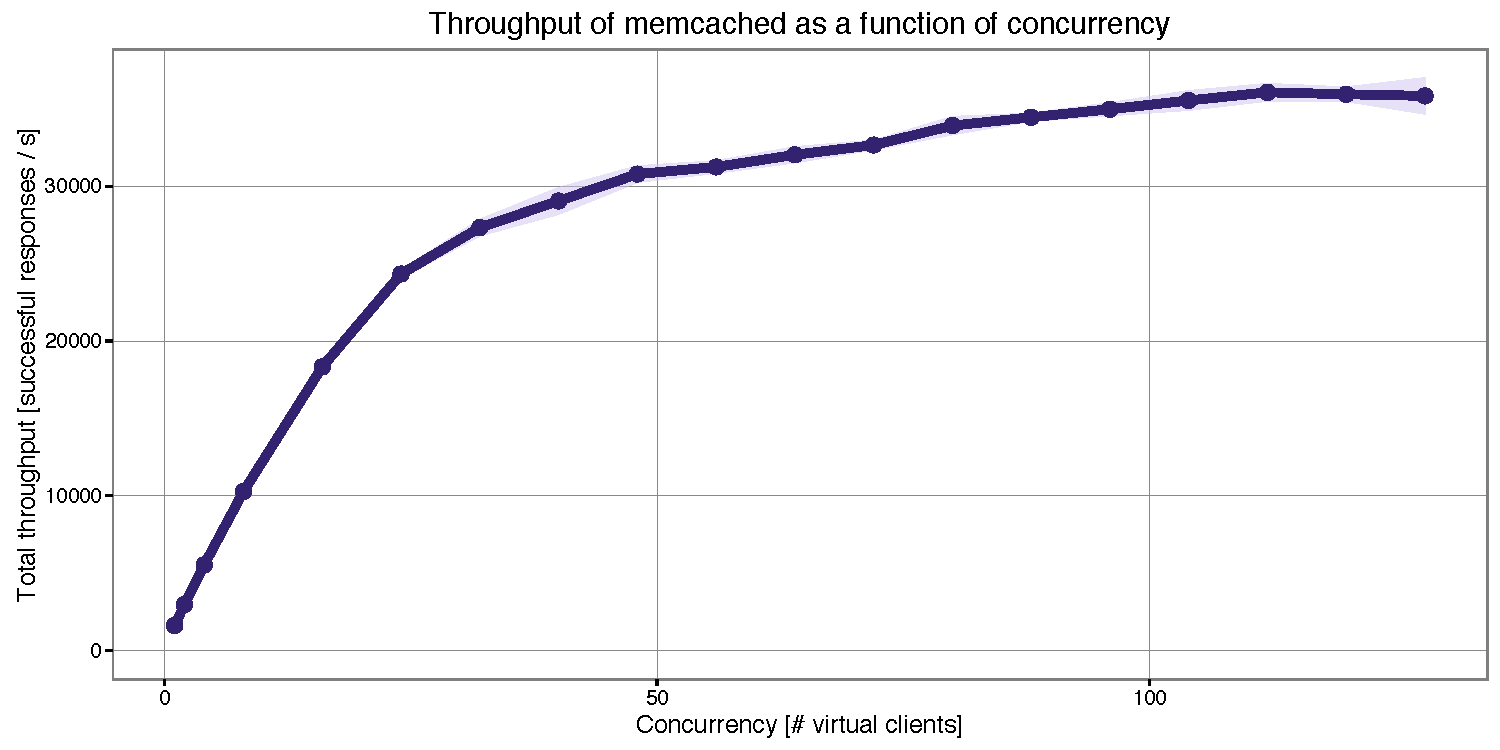
\includegraphics[width=\textwidth]{../results/baseline/graphs/throughput.pdf}
\label{fig:baseline:throughput}
\caption{Throughput of memcached without middleware, as measured by memaslap. Dark dots connected by a line show the mean throughput and the light ribbon surronding the line shows $\pm 1$ standard deviation of throughput over 5 repetitions.}
\end{figure}

\subsection{Response time}\label{sec:baseline:rt}

From Figure~\ref{fig:baseline:responsetime} we observe that response time grows slowly up to 24 virtual clients, from which point mean response time starts to grow linearly with the number of clients, and the standard deviation of response time increases significantly. The mean increases because memcached is unable to service all incoming requests immediately so some requests have to wait.

When the system starts to saturate, standard deviation also increases. \todo{WHY?} Statistical explanation: heavy tail for this distribution.



\todo{Explain high std: Upon examining logs manually, lalala distribution}

\begin{figure}[p]
\centering
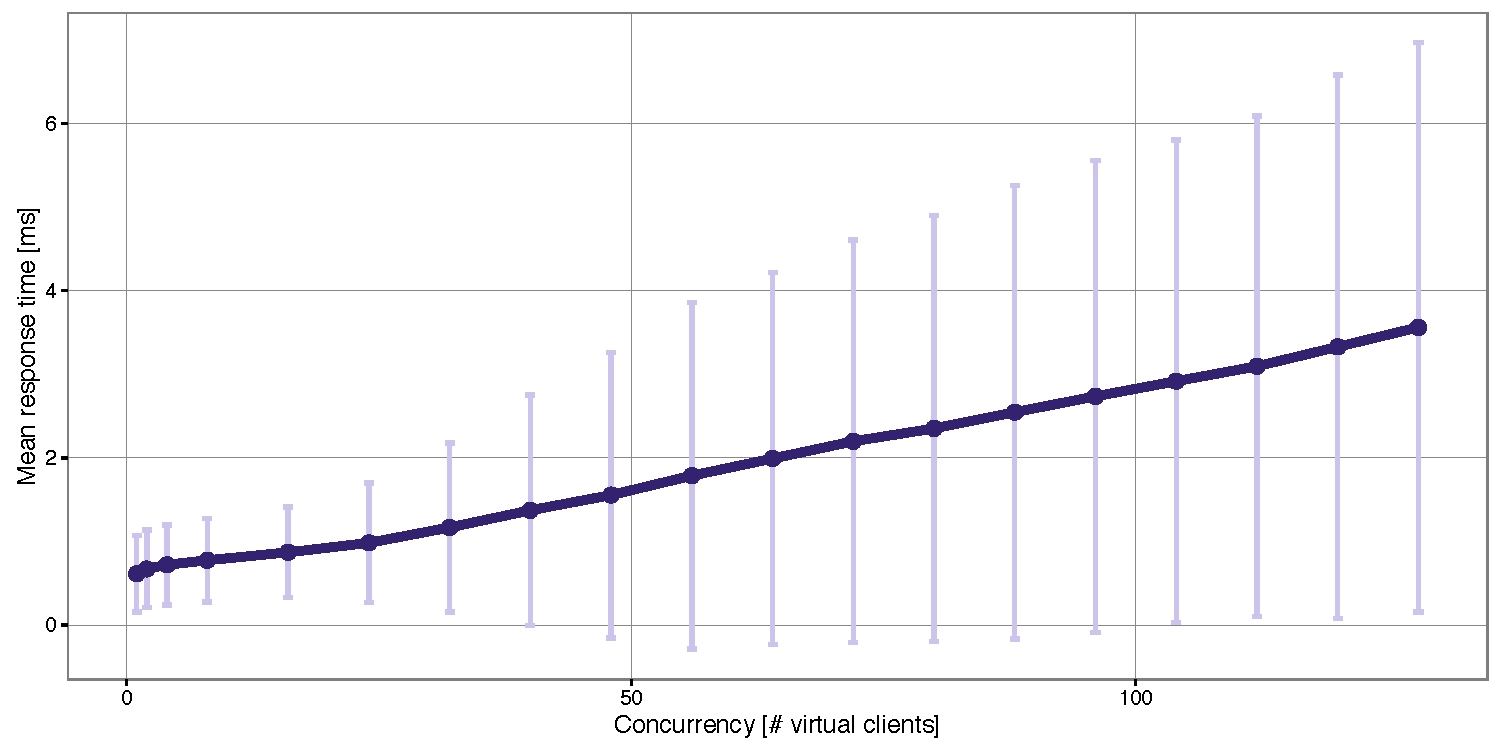
\includegraphics[width=\textwidth]{../results/baseline/graphs/responsetime.pdf}
\label{fig:baseline:responsetime}
\caption{Response time of memcached without middleware, as measured by memaslap. Dark dots connected by a line show the mean response time and the light ribbon surronding the line shows $\pm 1$ standard deviation aggregated over all requests sent with that concurrency. Standard deviation values from different repetitions were aggregated by a) calculating the variance for each repetitions, b) finding the weighted average of variance (where the weight is the number of successful requests in a repetition), and c) finding the square root of this sum. }
\end{figure}

\section{Stability Trace}\label{sec:trace}

\begin{center}
\small{
\smallskip
\begin{tabular}{|c|c|}
\hline Number of servers & 3 \\ 
\hline Number of client machines & 3 \\ 
\hline Virtual clients / machine &  64 \\ 
\hline Workload & Key 16B, Value 128B, Writes 1\% \\
\hline Middleware & Replicate to all ($R=3$) \\ 
\hline Runtime x repetitions & 65min x 1 \\ 
\hline Log files & trace-ms4, trace-ms5, trace-ms6, trace-mw, trace-req \\
\hline 
\end{tabular} }
\end{center}

The trace was run for 65 minutes; in the plots and analysis, the first three minutes and the last two minutes were removed to account for the warm-up and cool-down phase, respectively. The number of read threads per server was set to $T=5$ for the trace. Memaslap was set to record statistics in 30-second intervals.

The clients and the memcached server were run on Azure Basic\_A2 machines; the middleware was run on a Basic\_A4 instance. 
Both the middleware and memcached servers were accessed through their private IPs in the virtual network. Logs were parsed using Python and results plotted using R.



\subsection{Throughput}

From Figure~\ref{fig:rep3:throughput} we can see that the throughput remains at the same level of 7000 to 8000 operations per second throughout the whole experiment and thus the middleware can handle a long-running workload  without a degradation in performance. The variance can partly be explained by the random nature of the experiment: it is affected by the conditions (especially network conditions) on Azure. However, the sudden falls in throughput in the graph are likely to be caused by the Java garbage collector starting its operation.

We can use the Interactive Response Time Law to evaluate whether the results are reasonable. Given that in the trace (excluding warm-up and cool-down) the mean response time is $r=25.8$ms, the number of clients is $n = 3 \cdot 64 = 192$, and the clients can be assumed to have no think time ($z=0$), the predicted throughput is $\frac{n}{r + z} = 7430$ operations per second. This is well in line with the actual throughput of 7460 operations per second.

\begin{figure}[p]
\centering
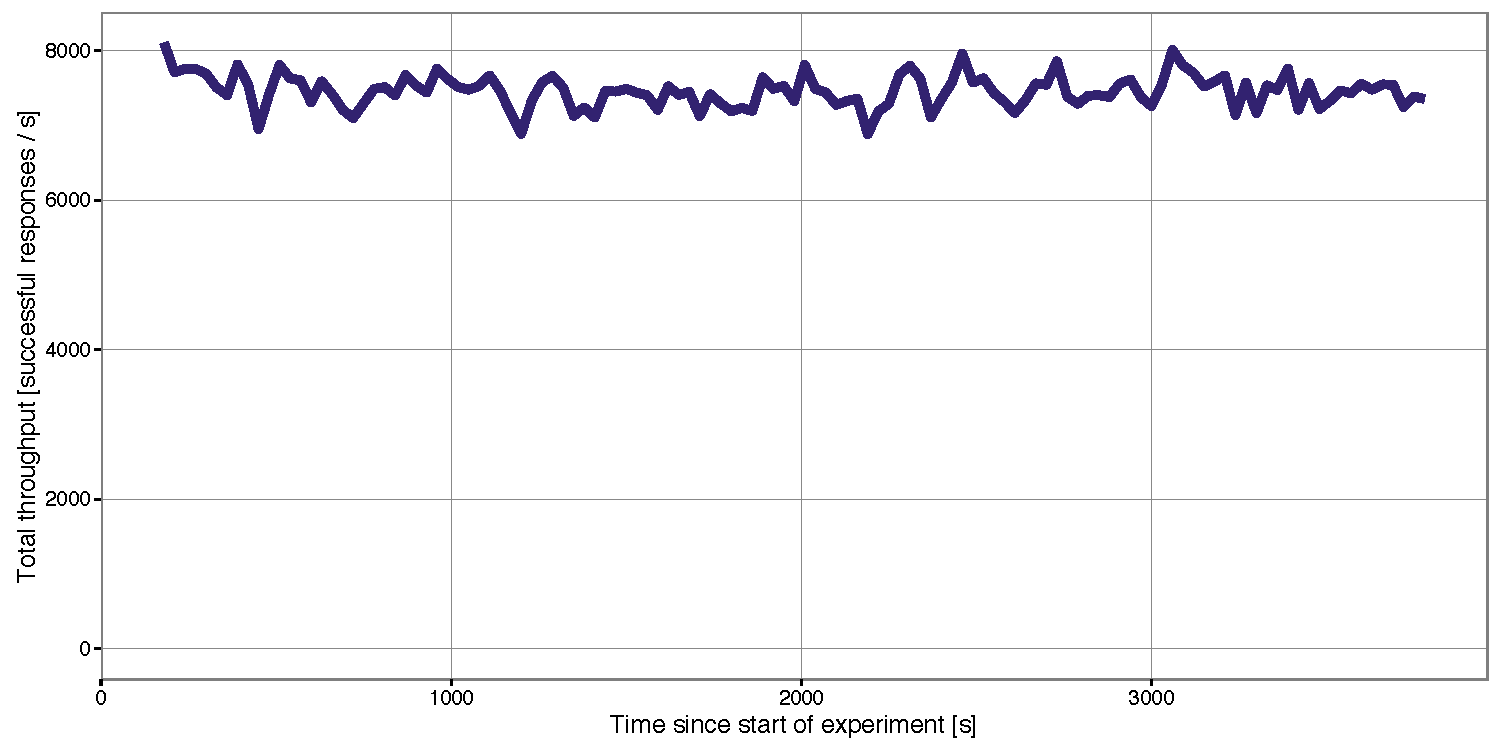
\includegraphics[width=\textwidth]{../results/trace_rep3/graphs/throughput.pdf}
\label{fig:rep3:throughput}
\caption{Throughput trace of the middleware. The dark line shows the total throughput, i.e. the sum over throughputs reported by the three clients.}
\end{figure}


\subsection{Response time}

Figure~\ref{fig:rep3:responsetime} shows that the response time stays constant around 25ms for the whole duration of the trace experiment.

\todo{explain why stdev is so high}

\begin{figure}[p]
\centering
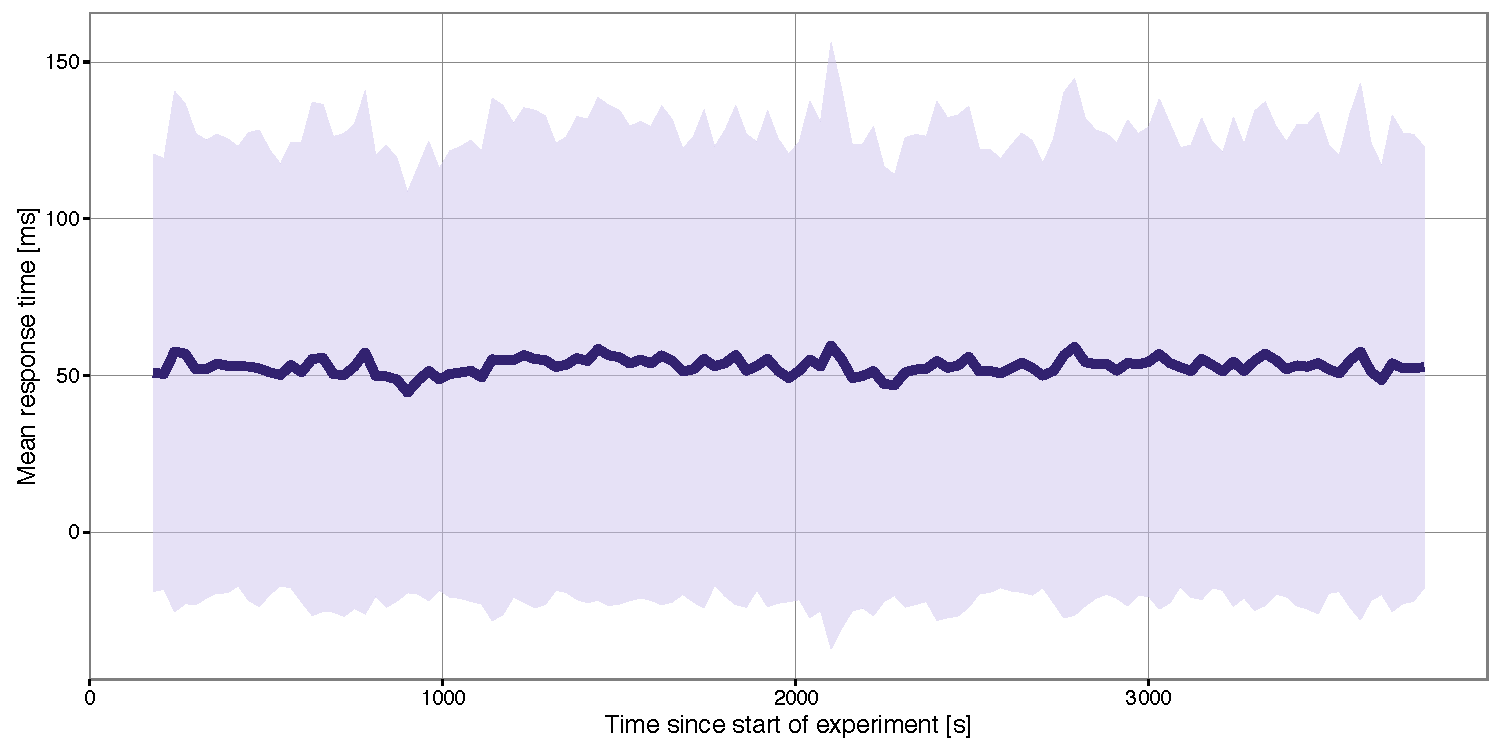
\includegraphics[width=\textwidth]{../results/trace_rep3/graphs/responsetime.pdf}
\label{fig:rep3:responsetime}
\caption{Response time trace of the middleware as measured by memaslap. The dark line shows the mean response time (calculated as the weighted average of mean response times reported by the three clients) and the light ribbon surrounding the line shows $\pm 1$ standard deviation. Standard deviation values from different repetitions were aggregated in the same way as in Section~\ref{sec:baseline}.}
\end{figure}

\subsection{Overhead of middleware}

In the trace experiment, three memcached servers need to service $3 \cdot 64 = 192$ clients, so the number of virtual clients per server is 64 (this assumes uniform load balancing, which was demonstrated in Section~\ref{sec:desc:hashing}). For this reason, we should compare the performance of the system with the performance of the baseline at 64 virtual clients. Since the trace is run with full replication, i.e. all writes are done to three servers instead of one, these two numbers are not be directly comparable. However, since write requests make up only 1\% of all requests, this difference is negligible.

The following table shows comparison of the baseline and actual (with middleware) performance of the system. Using the middleware introduces a roughly 4-fold decrease in throughput (decreasing it by 24540 requests per second) and roughly 12-fold increase in response time (adding 23.6 ms), which is a significant deterioration in performance.

\begin{center}
\begin{tabular}{|l|r|r|r|r|}
\hline \textbf{Metric }& \textbf{Baseline} & \textbf{Middleware} & \textbf{Overhead} & \textbf{Slow-down} \\ 
\hline throughput [requests/s] & 32000 & 7460 & -24540 & 4.3x \\ 
\hline response time [ms] & 2.2 & 25.8 & 23.6 & 11.7x \\ 
\hline 
\end{tabular} 
\end{center}


\pagebreak

\section*{Logfile listing}

\begin{tabular}{|c|l|}
\hline \textbf{Short name }& \textbf{Location} \\ 
\hline baseline-m*-c*-r* & \href{https://gitlab.inf.ethz.ch/pungast/asl-fall16-project/blob/master/results/baseline}{gitlab.inf.ethz.ch/.../results/baseline/baseline\_memaslap*\_conc*\_rep*.out} \\ 
\hline trace-ms4 & \resultsurl{trace\_rep3/memaslap4.out} \\ 
\hline trace-ms5 & \resultsurl{trace\_rep3/memaslap5.out} \\ 
\hline trace-ms6 & \resultsurl{trace\_rep3/memaslap6.out} \\ 
\hline trace-mw & \resultsurl{trace\_rep3/main.log} \\ 
\hline trace-req & \resultsurl{trace\_rep3/request.log} \\ 
\hline 
\end{tabular} 

\end{document}